\chapter{Présentation du projet}

\section{Hadoop et MapReduce}
Hadoop\cite{HadoopMapReduce} est une implémentation open source de MapReduce en Java distribuée par Apache.
 Les deux grandes parties de Hadoop sont:
\begin{itemize}
	\item Traitement des données: le framework MapReduce.
  	\item Stockage des données: Hadoop Distributed File System. 
 \end{itemize}
 Le principe est de distribuer les données (avec HDFS\footnote{Hadoop Distributed File System.}) et de faire des traitements sur ces données là où elles sont stockées (grâce à MapReduce) afin de paralléliser des opérations.

Hadoop exécute une tâche de en commençant par diviser les données en entrée en blocs de données de même taille. Ensuite, chaque bloc est planifié pour être exécuté.

\section{Contexte du projet}

Dans le cadre de notre projet de programmation, l'idée est de retranscrire la distribution des données en appliquant l'algorithme de mapReduce sans utiliser un framework\footnote{dont le plus connu est Hadoop} ou un système de gestion de fichiers.\\
Avec cela, le but est d'arriver à apporter une visualisation de la simulation sur un cluster de machines.

\textit{A noter: Dans le projet, il n'y a pas de cluster concret derrière. Notre travail est simplement de simuler le comportement de mapReduce sur des machines fictives qui n'existent pas sur un serveur ou autre support matériel.}\\

La représentation graphique doit comprendre les phases de map et de reduce, toutes les deux fournies comme fonctions par l'utilisateur de l'application. Il faut pouvoir visualiser les connections qui existent entre map et reduce sur les différentes machines.\\

L'objectif du projet est de déceler des bugs\footnote{en Français: bogue} dans la simulation.
Ces bugs peuvent correspondre à une mauvaise répartition des données dans l'ensemble  du cluster qui sont invisibles pour l'utilisateur. En effet, le retour du process de mapReduce est un ensemble de paires clé-valeur, il n'est pas possible de connaître quel processus fait quelle tâche ou quel processus ne fait rien. Grâce à VisualMapReduce, l'utilisateur peut voir visuellement s'il a donné par exemple un nombre de machines/coeurs important par rapport à ses données traitées et vis-versa.\\
Cette application, destinée à l'enseignement, permettra à des étudiants en Master 2 Informatique de simuler un cluster et comprendre le fonctionnement de MapReduce.

\section{Description détaillée du process de mapReduce}
\subsection{Notions importantes}

Avant de lister les différentes phases de mapReduce, il y a certaines notions importantes à savoir. Nous citons:\\

\begin{itemize}
\item {\bf Slot} : Le cluster d'éxécution comprends {\tt m} machines avec {\tt c} coeurs, ce qui représente {\bf m*c} slots d'éxécution.
Un slot peut accueillir un mapper ou un reducer. Le slot est libéré lorsque l'exécution du mapper ou reducer se termine.
\item {\bf Job}  : Un job est un ensemble de map et reduce. Il dispose en entrée d'un jeu de données.
\begin{figure}[H]
  \centering
    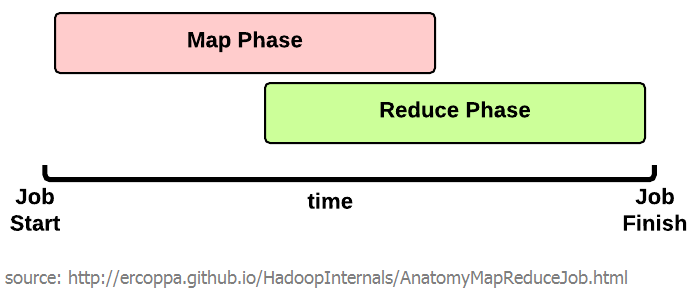
\includegraphics[scale=0.9]{images/job_timeline.png}
        \caption{Job dans mapReduce}
\end{figure}
\item {\bf Task} : On trouve des mapTasks et des reduceTasks. une phase de map comprend plusieurs mapTasks et pareil pour une phase de reduce.

\item {\bf Mapper/Reducer} : Ce sont les définitions des fonctions map et reduce. Un mapper est appliqué sur chaque slot. On a donc autant de mappers que de slots du cluster.\footnote{Il faut distinguer entre Mapper et MapTask. Un mapper peut accueillir plusieurs mapTasks. Une mapTask est une tache individuelle. Pour simplifier: un mapper = map+map+...+map}\\
Le mapper est appliqué sur chaque entrée du résultat de la fonction de découpage "split()" qui sera expliqué plus tard dans le document.  
Un reducer est appliqué sur toutes les valeurs associées aux mêmes clés générées.\\

Dans mapReduce, l'utilisateur définit un mapper et un reducer avec les signatures suivantes\cite{mapReduceTextProcessing}:
\[	map: (k_1,v_1) \rightarrow [(k_2,v_2)] \]
\[  reduce:(k_2,[v_2]) \rightarrow [(k_3,v_3)] \]
\end{itemize}

\subsection{Phases dans mapReduce}
L'algorithme MapReduce se décompose en plusieurs phases: {\bf Split, Map, Combine, Partition, Shuffle} et {\bf Reduce}.\\
\begin{itemize}
\item {\bf Split}: C'est une fonction qui récupère l'ensemble des données d'entrées et retourne des objets structurés qui serviront comme entrée de map. Dans la figure 1.2, l'étape de split répartie un fichier textuel selon son nombre de lignes.

\item {\bf Map}: Prend en entrée une ou plusieurs données. Les résultats sont stockés sous forme de paires <key, value> (<clé, valeur>) dites intermédiaires.

\item {\bf Combine}: Optionnel. Il possède les mêmes propriétés d'entrée/sortie que map. Son but est de faciliter la tâche de reduce en efectuant un "merge" partiel\cite{Google} sur les résultats du map.\\
Dans la figure 1.2, la phase de combine n'existait pas dans le schéma, mais dans le but de montrer son utilité, nous avons modifié la figure et rajouté le combiner à l'exemple.

\item {\bf Partition}: contrôle le partitionnement des clés des résultats de map. Par défaut, le partitioner utilise une fonction de hashage.Le nombre total de partitions est le même que le nombre des tâches de reduce. Le partitionneur intervient entre les phases de map et shuffle. Pour l'exemple de Wordcount de la figure 1.2, il agirait pour faire le partitionnement des sorties de {\tt map} sur les 4 reducers qui existent.


\item {\bf Shuffle}: C'est la phase de transfert des données des mappers aux reducers. Plus clairement, elle fournie les entrées de reduce.\\
Le shuffle est de la forme:
\[  shuffle:[(k_2,v_2)] \rightarrow (k_2,[v_2]) \]


\item {\bf Reduce}: C'est la phase de calcul du process. Elle accepte les clés intermédiaires et un ensemble de valeurs d'une même clé. Les valeurs sont alors traitées selon la fonction {\tt reduce} fournie.\\
\end{itemize}

Pour mieux comprendre l'exécution de mapReduce, nous proposons l'exemple de WordCount qui compte le nombre d'occurences des mots dans un texte.

\begin{figure}[H]
  \centering
    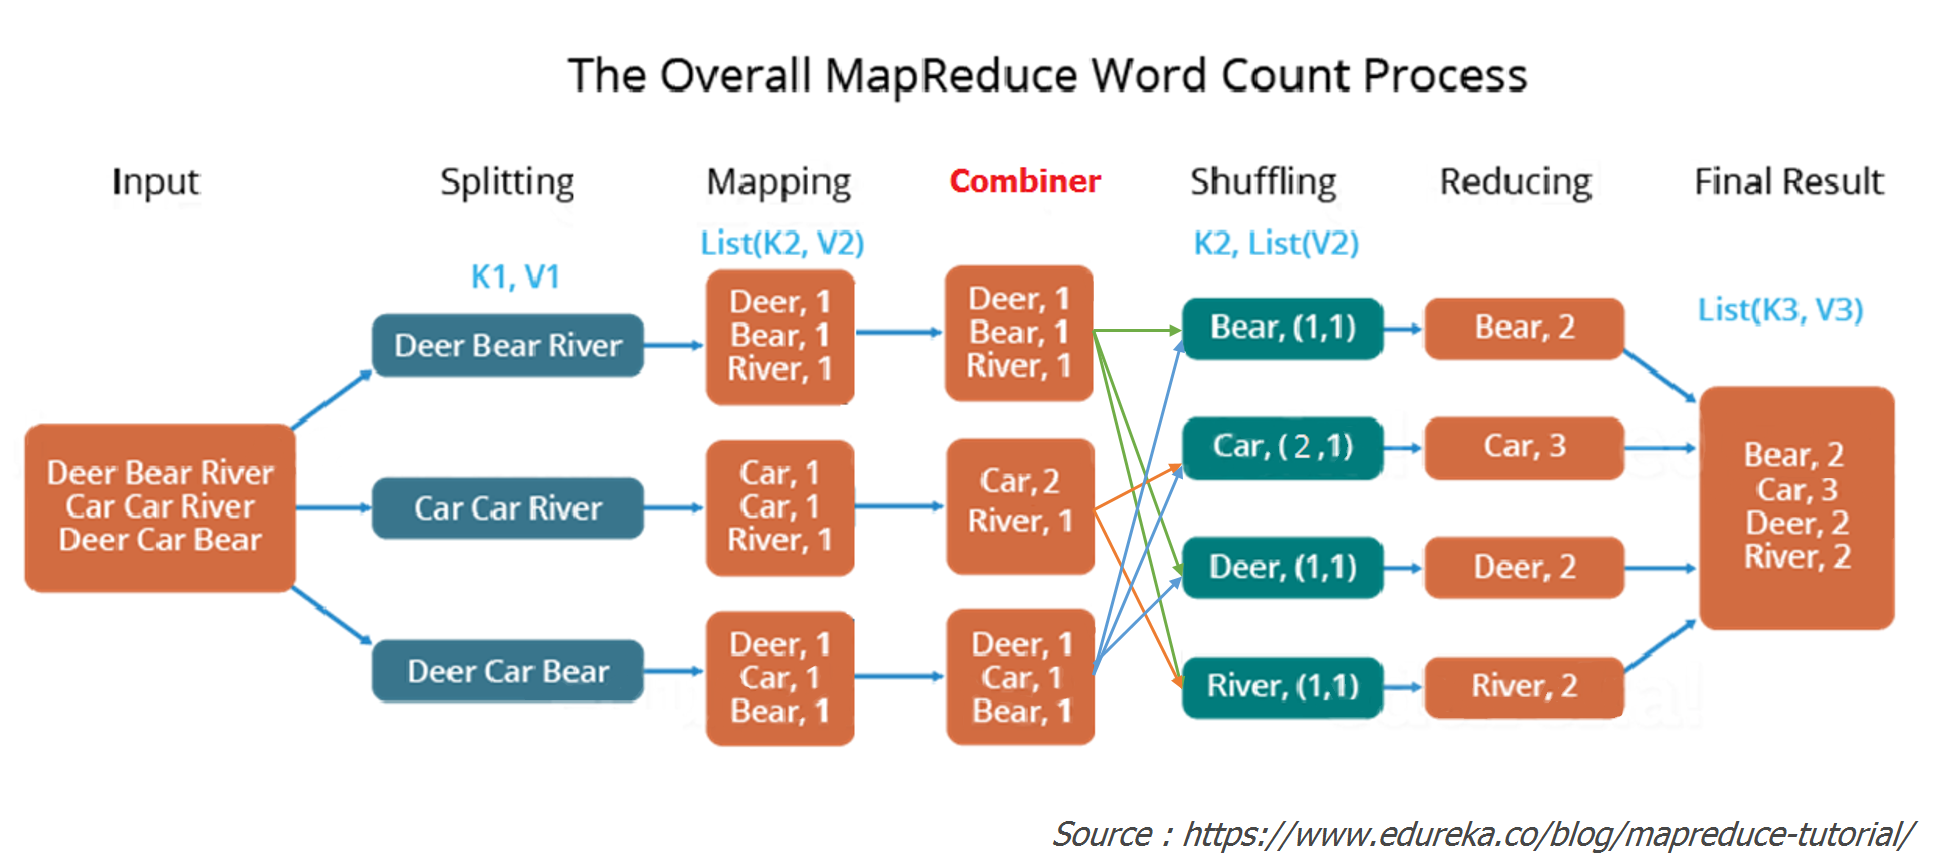
\includegraphics[scale=0.45]{images/mapreduce_process.png}
        \caption{Exemple MapReduce: WordCount}
\end{figure}

